% Generated by npm run evaluate; experiment selection-benchmark-v6-longitudinal.
\newcommand{\EvaluationSessions}{5985}
\newcommand{\EvaluationAnswers}{172088}
\newcommand{\EvaluationEvidenceEnds}{58}
\newcommand{\EvaluationNoQuestionEnds}{342}
\newcommand{\EvaluationBrierTable}{%
\begin{tabular}{llccc}
\hline
Situation & Sitzung & Zufall & Bewertungen + Lernstand & Informationsgewinn \\
\hline
Niedrig & 1 & \shortstack{$0{,}2294 \pm 0{,}0178$\\(0{,}2319)} & \shortstack{$0{,}2331 \pm 0{,}0226$\\(0{,}2347)} & \shortstack{$0{,}2346 \pm 0{,}0192$\\(0{,}2370)} \\
Niedrig & 2 & \shortstack{$0{,}2236 \pm 0{,}0271$\\(0{,}2416)} & \shortstack{$0{,}2313 \pm 0{,}0243$\\(0{,}2388)} & \shortstack{$0{,}2340 \pm 0{,}0217$\\(0{,}2380)} \\
Niedrig & 3 & \shortstack{$0{,}2195 \pm 0{,}0286$\\(0{,}2501)} & \shortstack{$0{,}2344 \pm 0{,}0261$\\(0{,}2411)} & \shortstack{$0{,}2334 \pm 0{,}0199$\\(0{,}2411)} \\
Niedrig & 4 & \shortstack{$0{,}2016 \pm 0{,}0368$\\(0{,}2571)} & \shortstack{$0{,}2341 \pm 0{,}0287$\\(0{,}2434)} & \shortstack{$0{,}2310 \pm 0{,}0288$\\(0{,}2443)} \\
Niedrig & 5 & \shortstack{$0{,}1945 \pm 0{,}0439$\\(0{,}2622)} & \shortstack{$0{,}2308 \pm 0{,}0270$\\(0{,}2454)} & \shortstack{$0{,}2309 \pm 0{,}0280$\\(0{,}2485)} \\
Gemischt & 1 & \shortstack{$0{,}2366 \pm 0{,}0187$\\(0{,}2499)} & \shortstack{$0{,}2343 \pm 0{,}0224$\\(0{,}2501)} & \shortstack{$0{,}2329 \pm 0{,}0179$\\(0{,}2519)} \\
Gemischt & 2 & \shortstack{$0{,}2117 \pm 0{,}0258$\\(0{,}2572)} & \shortstack{$0{,}2322 \pm 0{,}0223$\\(0{,}2527)} & \shortstack{$0{,}2322 \pm 0{,}0215$\\(0{,}2506)} \\
Gemischt & 3 & \shortstack{$0{,}1994 \pm 0{,}0308$\\(0{,}2633)} & \shortstack{$0{,}2330 \pm 0{,}0243$\\(0{,}2493)} & \shortstack{$0{,}2303 \pm 0{,}0217$\\(0{,}2522)} \\
Gemischt & 4 & \shortstack{$0{,}1771 \pm 0{,}0399$\\(0{,}2695)} & \shortstack{$0{,}2288 \pm 0{,}0250$\\(0{,}2492)} & \shortstack{$0{,}2271 \pm 0{,}0278$\\(0{,}2514)} \\
Gemischt & 5 & \shortstack{$0{,}1695 \pm 0{,}0435$\\(0{,}2718)} & \shortstack{$0{,}2259 \pm 0{,}0253$\\(0{,}2501)} & \shortstack{$0{,}2289 \pm 0{,}0293$\\(0{,}2498)} \\
Hoch & 1 & \shortstack{$0{,}2486 \pm 0{,}0187$\\(0{,}2861)} & \shortstack{$0{,}2266 \pm 0{,}0173$\\(0{,}2852)} & \shortstack{$0{,}2322 \pm 0{,}0186$\\(0{,}2845)} \\
Hoch & 2 & \shortstack{$0{,}1862 \pm 0{,}0280$\\(0{,}2884)} & \shortstack{$0{,}2281 \pm 0{,}0185$\\(0{,}2832)} & \shortstack{$0{,}2235 \pm 0{,}0153$\\(0{,}2850)} \\
Hoch & 3 & \shortstack{$0{,}1546 \pm 0{,}0385$\\(0{,}2887)} & \shortstack{$0{,}2195 \pm 0{,}0170$\\(0{,}2805)} & \shortstack{$0{,}2162 \pm 0{,}0193$\\(0{,}2827)} \\
Hoch & 4 & \shortstack{$0{,}1272 \pm 0{,}0418$\\(0{,}2913)} & \shortstack{$0{,}1979 \pm 0{,}0374$\\(0{,}2733)} & \shortstack{$0{,}2065 \pm 0{,}0423$\\(0{,}2679)} \\
Hoch & 5 & \shortstack{$0{,}1193 \pm 0{,}0461$\\(0{,}2922)} & \shortstack{$0{,}2269 \pm 0{,}0763_{n=89}$\\(0{,}2622)} & \shortstack{$0{,}1981 \pm 0{,}0785_{n=96}$\\(0{,}2635)} \\
Abweichend & 1 & \shortstack{$0{,}2478 \pm 0{,}0225$\\(0{,}2507)} & \shortstack{$0{,}2462 \pm 0{,}0279$\\(0{,}2484)} & \shortstack{$0{,}2468 \pm 0{,}0216$\\(0{,}2511)} \\
Abweichend & 2 & \shortstack{$0{,}2467 \pm 0{,}0283$\\(0{,}2531)} & \shortstack{$0{,}2487 \pm 0{,}0268$\\(0{,}2499)} & \shortstack{$0{,}2488 \pm 0{,}0293$\\(0{,}2482)} \\
Abweichend & 3 & \shortstack{$0{,}2465 \pm 0{,}0426$\\(0{,}2536)} & \shortstack{$0{,}2446 \pm 0{,}0314$\\(0{,}2468)} & \shortstack{$0{,}2488 \pm 0{,}0274$\\(0{,}2486)} \\
Abweichend & 4 & \shortstack{$0{,}2423 \pm 0{,}0406$\\(0{,}2555)} & \shortstack{$0{,}2505 \pm 0{,}0267$\\(0{,}2436)} & \shortstack{$0{,}2529 \pm 0{,}0333$\\(0{,}2463)} \\
Abweichend & 5 & \shortstack{$0{,}2345 \pm 0{,}0432$\\(0{,}2566)} & \shortstack{$0{,}2454 \pm 0{,}0303$\\(0{,}2443)} & \shortstack{$0{,}2447 \pm 0{,}0301$\\(0{,}2404)} \\
\hline
\end{tabular}}
\newcommand{\EvaluationLogLossTable}{%
\begin{tabular}{llccc}
\hline
Situation & Sitzung & Zufall & Bewertungen + Lernstand & Informationsgewinn \\
\hline
Niedrig & 1 & \shortstack{$0{,}6521 \pm 0{,}0382$\\(0{,}6567)} & \shortstack{$0{,}6601 \pm 0{,}0474$\\(0{,}6625)} & \shortstack{$0{,}6630 \pm 0{,}0402$\\(0{,}6671)} \\
Niedrig & 2 & \shortstack{$0{,}6388 \pm 0{,}0604$\\(0{,}6763)} & \shortstack{$0{,}6561 \pm 0{,}0507$\\(0{,}6707)} & \shortstack{$0{,}6618 \pm 0{,}0455$\\(0{,}6690)} \\
Niedrig & 3 & \shortstack{$0{,}6292 \pm 0{,}0659$\\(0{,}6933)} & \shortstack{$0{,}6621 \pm 0{,}0542$\\(0{,}6754)} & \shortstack{$0{,}6605 \pm 0{,}0416$\\(0{,}6754)} \\
Niedrig & 4 & \shortstack{$0{,}5849 \pm 0{,}0854$\\(0{,}7073)} & \shortstack{$0{,}6616 \pm 0{,}0596$\\(0{,}6799)} & \shortstack{$0{,}6553 \pm 0{,}0600$\\(0{,}6817)} \\
Niedrig & 5 & \shortstack{$0{,}5728 \pm 0{,}1070$\\(0{,}7176)} & \shortstack{$0{,}6544 \pm 0{,}0560$\\(0{,}6838)} & \shortstack{$0{,}6544 \pm 0{,}0581$\\(0{,}6901)} \\
Gemischt & 1 & \shortstack{$0{,}6651 \pm 0{,}0401$\\(0{,}6930)} & \shortstack{$0{,}6611 \pm 0{,}0474$\\(0{,}6933)} & \shortstack{$0{,}6578 \pm 0{,}0376$\\(0{,}6970)} \\
Gemischt & 2 & \shortstack{$0{,}6103 \pm 0{,}0594$\\(0{,}7076)} & \shortstack{$0{,}6564 \pm 0{,}0467$\\(0{,}6985)} & \shortstack{$0{,}6568 \pm 0{,}0454$\\(0{,}6944)} \\
Gemischt & 3 & \shortstack{$0{,}5829 \pm 0{,}0742$\\(0{,}7199)} & \shortstack{$0{,}6585 \pm 0{,}0509$\\(0{,}6917)} & \shortstack{$0{,}6529 \pm 0{,}0454$\\(0{,}6976)} \\
Gemischt & 4 & \shortstack{$0{,}5276 \pm 0{,}0953$\\(0{,}7322)} & \shortstack{$0{,}6498 \pm 0{,}0522$\\(0{,}6916)} & \shortstack{$0{,}6459 \pm 0{,}0582$\\(0{,}6961)} \\
Gemischt & 5 & \shortstack{$0{,}5133 \pm 0{,}1089$\\(0{,}7369)} & \shortstack{$0{,}6436 \pm 0{,}0526$\\(0{,}6933)} & \shortstack{$0{,}6500 \pm 0{,}0607$\\(0{,}6927)} \\
Hoch & 1 & \shortstack{$0{,}6863 \pm 0{,}0412$\\(0{,}7656)} & \shortstack{$0{,}6413 \pm 0{,}0370$\\(0{,}7639)} & \shortstack{$0{,}6531 \pm 0{,}0396$\\(0{,}7624)} \\
Hoch & 2 & \shortstack{$0{,}5495 \pm 0{,}0663$\\(0{,}7704)} & \shortstack{$0{,}6448 \pm 0{,}0396$\\(0{,}7598)} & \shortstack{$0{,}6350 \pm 0{,}0327$\\(0{,}7634)} \\
Hoch & 3 & \shortstack{$0{,}4794 \pm 0{,}0958$\\(0{,}7710)} & \shortstack{$0{,}6271 \pm 0{,}0361$\\(0{,}7544)} & \shortstack{$0{,}6199 \pm 0{,}0411$\\(0{,}7588)} \\
Hoch & 4 & \shortstack{$0{,}4115 \pm 0{,}1058$\\(0{,}7761)} & \shortstack{$0{,}5823 \pm 0{,}0795$\\(0{,}7400)} & \shortstack{$0{,}6006 \pm 0{,}0899$\\(0{,}7291)} \\
Hoch & 5 & \shortstack{$0{,}3948 \pm 0{,}1197$\\(0{,}7779)} & \shortstack{$0{,}6460 \pm 0{,}1603_{n=89}$\\(0{,}7176)} & \shortstack{$0{,}5854 \pm 0{,}1660_{n=96}$\\(0{,}7202)} \\
Abweichend & 1 & \shortstack{$0{,}6899 \pm 0{,}0488$\\(0{,}6945)} & \shortstack{$0{,}6865 \pm 0{,}0590$\\(0{,}6900)} & \shortstack{$0{,}6875 \pm 0{,}0456$\\(0{,}6953)} \\
Abweichend & 2 & \shortstack{$0{,}6908 \pm 0{,}0644$\\(0{,}6994)} & \shortstack{$0{,}6916 \pm 0{,}0567$\\(0{,}6930)} & \shortstack{$0{,}6919 \pm 0{,}0619$\\(0{,}6896)} \\
Abweichend & 3 & \shortstack{$0{,}6961 \pm 0{,}1017$\\(0{,}7003)} & \shortstack{$0{,}6831 \pm 0{,}0657$\\(0{,}6866)} & \shortstack{$0{,}6919 \pm 0{,}0576$\\(0{,}6904)} \\
Abweichend & 4 & \shortstack{$0{,}6878 \pm 0{,}1005$\\(0{,}7042)} & \shortstack{$0{,}6955 \pm 0{,}0558$\\(0{,}6803)} & \shortstack{$0{,}7009 \pm 0{,}0700$\\(0{,}6858)} \\
Abweichend & 5 & \shortstack{$0{,}6720 \pm 0{,}1064$\\(0{,}7064)} & \shortstack{$0{,}6850 \pm 0{,}0633$\\(0{,}6816)} & \shortstack{$0{,}6837 \pm 0{,}0633$\\(0{,}6739)} \\
\hline
\end{tabular}}
\newcommand{\EvaluationNeedTable}{%
\begin{tabular}{llccc}
\hline
Situation & Sitzung & Zufall & Bewertungen + Lernstand & Informationsgewinn \\
\hline
Niedrig & 1 & \shortstack{$84{,}3 \pm 6{,}5$} & \shortstack{$79{,}9 \pm 8{,}4$} & \shortstack{$78{,}3 \pm 7{,}9$} \\
Niedrig & 2 & \shortstack{$71{,}9 \pm 9{,}3$} & \shortstack{$76{,}3 \pm 9{,}2$} & \shortstack{$76{,}8 \pm 8{,}5$} \\
Niedrig & 3 & \shortstack{$61{,}7 \pm 9{,}0$} & \shortstack{$73{,}8 \pm 9{,}5$} & \shortstack{$73{,}1 \pm 7{,}4$} \\
Niedrig & 4 & \shortstack{$52{,}1 \pm 9{,}1$} & \shortstack{$70{,}9 \pm 10{,}5$} & \shortstack{$68{,}1 \pm 10{,}3$} \\
Niedrig & 5 & \shortstack{$46{,}7 \pm 8{,}7$} & \shortstack{$67{,}9 \pm 10{,}7$} & \shortstack{$64{,}7 \pm 9{,}8$} \\
Gemischt & 1 & \shortstack{$61{,}1 \pm 7{,}5$} & \shortstack{$61{,}5 \pm 10{,}8$} & \shortstack{$58{,}9 \pm 9{,}0$} \\
Gemischt & 2 & \shortstack{$51{,}8 \pm 10{,}2$} & \shortstack{$59{,}4 \pm 9{,}1$} & \shortstack{$60{,}9 \pm 8{,}7$} \\
Gemischt & 3 & \shortstack{$44{,}1 \pm 9{,}1$} & \shortstack{$63{,}0 \pm 10{,}7$} & \shortstack{$58{,}8 \pm 7{,}9$} \\
Gemischt & 4 & \shortstack{$36{,}5 \pm 8{,}7$} & \shortstack{$61{,}9 \pm 12{,}4$} & \shortstack{$60{,}4 \pm 12{,}3$} \\
Gemischt & 5 & \shortstack{$34{,}4 \pm 8{,}0$} & \shortstack{$60{,}7 \pm 11{,}4$} & \shortstack{$62{,}3 \pm 11{,}4$} \\
Hoch & 1 & \shortstack{$14{,}1 \pm 6{,}3$} & \shortstack{$15{,}4 \pm 8{,}5$} & \shortstack{$16{,}5 \pm 6{,}3$} \\
Hoch & 2 & \shortstack{$11{,}5 \pm 5{,}8$} & \shortstack{$17{,}5 \pm 8{,}6$} & \shortstack{$15{,}8 \pm 6{,}6$} \\
Hoch & 3 & \shortstack{$10{,}0 \pm 4{,}6$} & \shortstack{$21{,}2 \pm 10{,}4$} & \shortstack{$18{,}3 \pm 8{,}3$} \\
Hoch & 4 & \shortstack{$8{,}1 \pm 5{,}4$} & \shortstack{$33{,}1 \pm 15{,}9$} & \shortstack{$38{,}4 \pm 17{,}2$} \\
Hoch & 5 & \shortstack{$7{,}0 \pm 5{,}2$} & \shortstack{$46{,}7 \pm 35{,}5_{n=89}$} & \shortstack{$45{,}0 \pm 30{,}8_{n=96}$} \\
Abweichend & 1 & \shortstack{$63{,}7 \pm 7{,}1$} & \shortstack{$66{,}9 \pm 11{,}7$} & \shortstack{$64{,}7 \pm 8{,}1$} \\
Abweichend & 2 & \shortstack{$60{,}5 \pm 9{,}7$} & \shortstack{$67{,}5 \pm 10{,}0$} & \shortstack{$68{,}0 \pm 8{,}0$} \\
Abweichend & 3 & \shortstack{$58{,}4 \pm 9{,}0$} & \shortstack{$71{,}8 \pm 10{,}8$} & \shortstack{$68{,}4 \pm 9{,}0$} \\
Abweichend & 4 & \shortstack{$55{,}0 \pm 10{,}4$} & \shortstack{$76{,}4 \pm 10{,}1$} & \shortstack{$76{,}3 \pm 11{,}2$} \\
Abweichend & 5 & \shortstack{$54{,}8 \pm 10{,}5$} & \shortstack{$79{,}2 \pm 10{,}9$} & \shortstack{$81{,}5 \pm 8{,}9$} \\
\hline
\end{tabular}}
\newcommand{\EvaluationCoverageTable}{%
\begin{tabular}{llccc}
\hline
Situation & Sitzung & Zufall & Bewertungen + Lernstand & Informationsgewinn \\
\hline
Niedrig & 1 & \shortstack{$55{,}4 \pm 4{,}7$} & \shortstack{$29{,}9 \pm 2{,}0$} & \shortstack{$33{,}2 \pm 1{,}0$} \\
Niedrig & 2 & \shortstack{$55{,}5 \pm 4{,}9$} & \shortstack{$30{,}5 \pm 2{,}1$} & \shortstack{$29{,}1 \pm 1{,}8$} \\
Niedrig & 3 & \shortstack{$55{,}8 \pm 4{,}3$} & \shortstack{$31{,}1 \pm 2{,}6$} & \shortstack{$28{,}2 \pm 2{,}7$} \\
Niedrig & 4 & \shortstack{$55{,}9 \pm 4{,}2$} & \shortstack{$32{,}3 \pm 3{,}2$} & \shortstack{$32{,}5 \pm 4{,}0$} \\
Niedrig & 5 & \shortstack{$56{,}2 \pm 4{,}6$} & \shortstack{$32{,}8 \pm 3{,}5$} & \shortstack{$33{,}4 \pm 3{,}5$} \\
Gemischt & 1 & \shortstack{$55{,}4 \pm 4{,}7$} & \shortstack{$31{,}7 \pm 2{,}3$} & \shortstack{$34{,}7 \pm 1{,}5$} \\
Gemischt & 2 & \shortstack{$55{,}5 \pm 4{,}9$} & \shortstack{$32{,}4 \pm 2{,}2$} & \shortstack{$30{,}4 \pm 1{,}9$} \\
Gemischt & 3 & \shortstack{$55{,}8 \pm 4{,}3$} & \shortstack{$32{,}3 \pm 2{,}8$} & \shortstack{$30{,}4 \pm 3{,}2$} \\
Gemischt & 4 & \shortstack{$55{,}9 \pm 4{,}2$} & \shortstack{$33{,}5 \pm 3{,}2$} & \shortstack{$34{,}7 \pm 3{,}8$} \\
Gemischt & 5 & \shortstack{$56{,}2 \pm 4{,}6$} & \shortstack{$33{,}5 \pm 3{,}7$} & \shortstack{$31{,}4 \pm 3{,}0$} \\
Hoch & 1 & \shortstack{$55{,}4 \pm 4{,}7$} & \shortstack{$36{,}4 \pm 2{,}4$} & \shortstack{$38{,}5 \pm 1{,}6$} \\
Hoch & 2 & \shortstack{$55{,}5 \pm 4{,}9$} & \shortstack{$36{,}2 \pm 2{,}4$} & \shortstack{$34{,}8 \pm 1{,}8$} \\
Hoch & 3 & \shortstack{$55{,}8 \pm 4{,}3$} & \shortstack{$37{,}0 \pm 2{,}8$} & \shortstack{$36{,}7 \pm 3{,}7$} \\
Hoch & 4 & \shortstack{$55{,}9 \pm 4{,}2$} & \shortstack{$23{,}3 \pm 6{,}6$} & \shortstack{$20{,}7 \pm 6{,}6$} \\
Hoch & 5 & \shortstack{$56{,}2 \pm 4{,}6$} & \shortstack{$6{,}3 \pm 2{,}9_{n=89}$} & \shortstack{$6{,}4 \pm 3{,}0_{n=96}$} \\
Abweichend & 1 & \shortstack{$55{,}4 \pm 4{,}7$} & \shortstack{$31{,}3 \pm 2{,}2$} & \shortstack{$34{,}5 \pm 1{,}4$} \\
Abweichend & 2 & \shortstack{$55{,}5 \pm 4{,}9$} & \shortstack{$31{,}4 \pm 2{,}5$} & \shortstack{$29{,}8 \pm 1{,}9$} \\
Abweichend & 3 & \shortstack{$55{,}8 \pm 4{,}3$} & \shortstack{$31{,}7 \pm 2{,}9$} & \shortstack{$29{,}5 \pm 2{,}7$} \\
Abweichend & 4 & \shortstack{$55{,}9 \pm 4{,}2$} & \shortstack{$31{,}5 \pm 2{,}7$} & \shortstack{$31{,}5 \pm 4{,}2$} \\
Abweichend & 5 & \shortstack{$56{,}2 \pm 4{,}6$} & \shortstack{$32{,}6 \pm 3{,}4$} & \shortstack{$31{,}5 \pm 4{,}1$} \\
\hline
\end{tabular}}
\newcommand{\EvaluationBrierPlot}{%
\begin{minipage}{0.48\textwidth}\centering
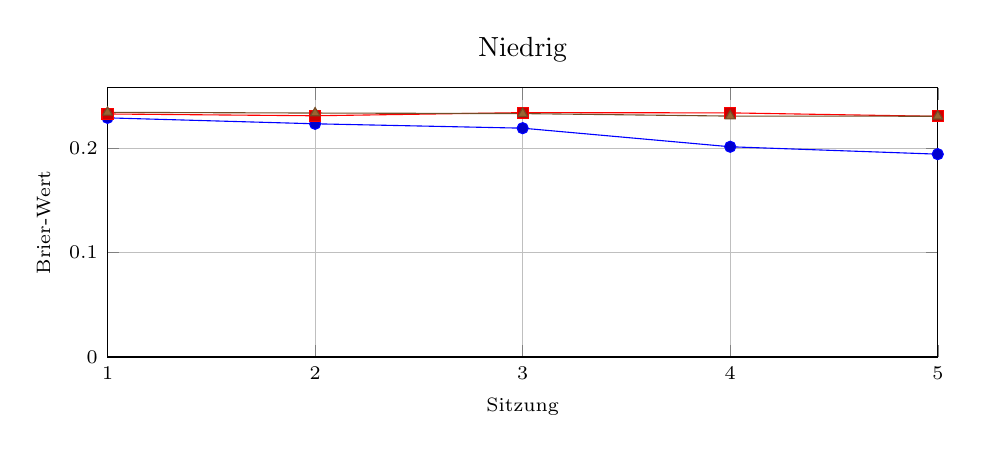
\begin{tikzpicture}
\begin{axis}[width=\linewidth,height=5cm,title={Niedrig},xlabel={Sitzung},ylabel={Brier-Wert},xmin=1,xmax=5,xtick={1,...,5},ymin=0,grid=major,tick label style={font=\scriptsize},label style={font=\scriptsize}]
\addplot+[mark=*] coordinates {(1,0.2293557905706794) (2,0.22364771448643328) (3,0.2194514148809096) (4,0.20162621727871696) (5,0.19453200828826817)};
\addplot+[mark=square*] coordinates {(1,0.2330602533533862) (2,0.23133767483012324) (3,0.23435955663651437) (4,0.23412277943027376) (5,0.2307897265802123)};
\addplot+[mark=triangle*] coordinates {(1,0.2346311771452502) (2,0.2339698470370803) (3,0.23343908924959542) (4,0.23104178363358358) (5,0.23091424368036179)};
\end{axis}
\end{tikzpicture}
\end{minipage}\hfill
\begin{minipage}{0.48\textwidth}\centering
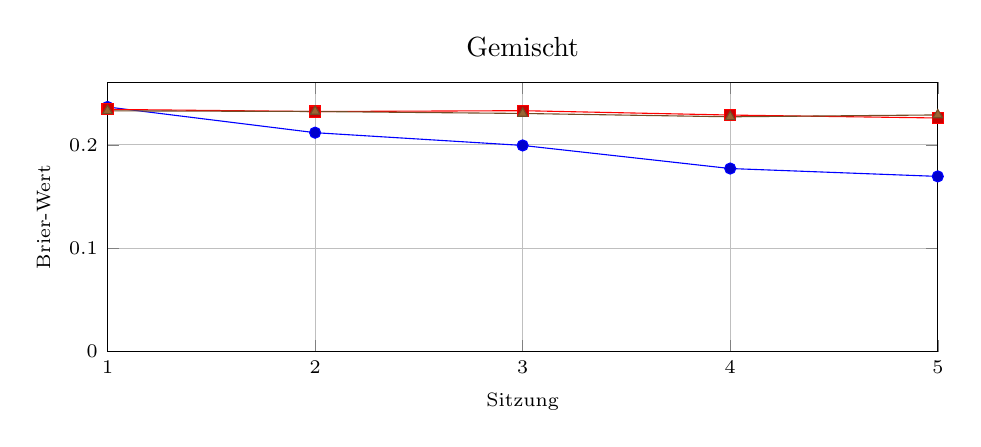
\begin{tikzpicture}
\begin{axis}[width=\linewidth,height=5cm,title={Gemischt},xlabel={Sitzung},ylabel={Brier-Wert},xmin=1,xmax=5,xtick={1,...,5},ymin=0,grid=major,tick label style={font=\scriptsize},label style={font=\scriptsize}]
\addplot+[mark=*] coordinates {(1,0.23659261645741989) (2,0.2117290140448366) (3,0.19939482043392354) (4,0.17706689338909865) (5,0.16946092824650208)};
\addplot+[mark=square*] coordinates {(1,0.23425022814843785) (2,0.23217843935351873) (3,0.2330022165635759) (4,0.22877644712011275) (5,0.2259276641329822)};
\addplot+[mark=triangle*] coordinates {(1,0.23285340846766617) (2,0.2322123472892886) (3,0.2303090635648175) (4,0.22708617735731604) (5,0.22889040472257885)};
\end{axis}
\end{tikzpicture}
\end{minipage}\par\medskip
\begin{minipage}{0.48\textwidth}\centering
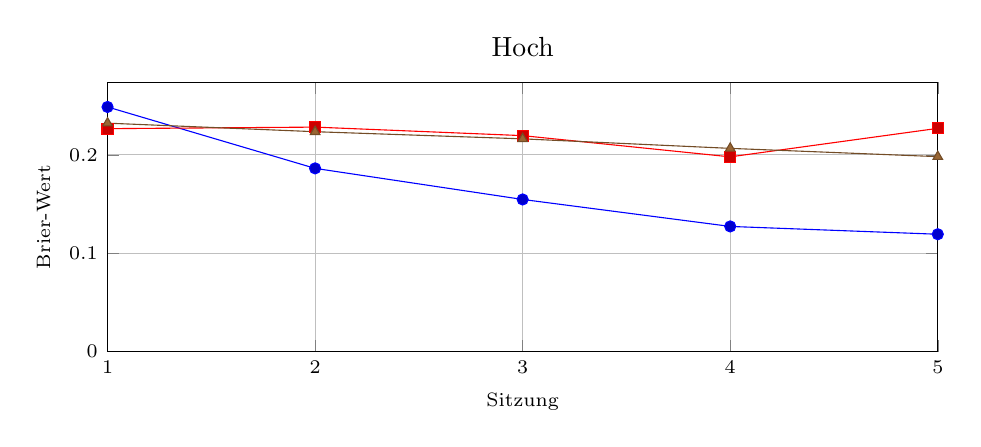
\begin{tikzpicture}
\begin{axis}[width=\linewidth,height=5cm,title={Hoch},xlabel={Sitzung},ylabel={Brier-Wert},xmin=1,xmax=5,xtick={1,...,5},ymin=0,grid=major,tick label style={font=\scriptsize},label style={font=\scriptsize}]
\addplot+[mark=*] coordinates {(1,0.2486125466728814) (2,0.18622587094282975) (3,0.15464667350259498) (4,0.12723364398659576) (5,0.11930203829748738)};
\addplot+[mark=square*] coordinates {(1,0.2265662320386342) (2,0.22814723889462907) (3,0.21948839492136155) (4,0.19792579881781353) (5,0.22689122448092375)};
\addplot+[mark=triangle*] coordinates {(1,0.23216212089000327) (2,0.22348240630387678) (3,0.21622082045548371) (4,0.2065396558554648) (5,0.19814060852529122)};
\end{axis}
\end{tikzpicture}
\end{minipage}\hfill
\begin{minipage}{0.48\textwidth}\centering
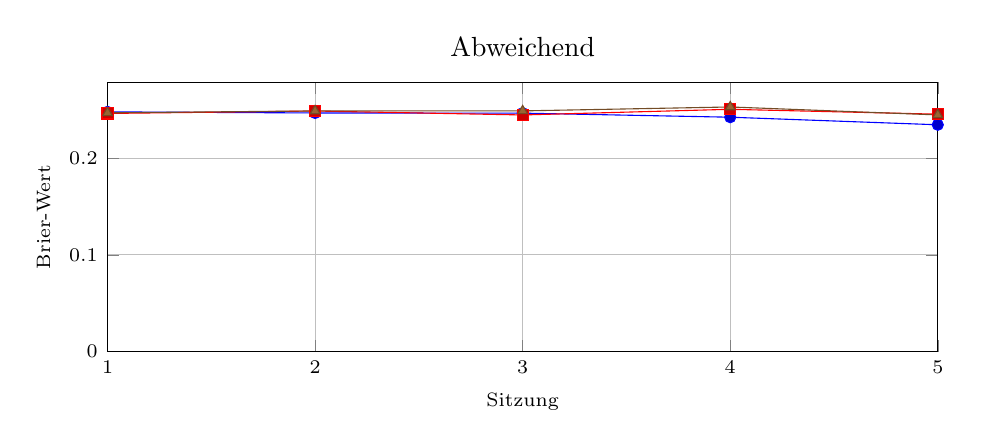
\begin{tikzpicture}
\begin{axis}[width=\linewidth,height=5cm,title={Abweichend},xlabel={Sitzung},ylabel={Brier-Wert},xmin=1,xmax=5,xtick={1,...,5},ymin=0,grid=major,tick label style={font=\scriptsize},label style={font=\scriptsize}]
\addplot+[mark=*] coordinates {(1,0.24782296154360683) (2,0.24669535762636016) (3,0.24651617661940498) (4,0.24230566095163297) (5,0.2344835494682723)};
\addplot+[mark=square*] coordinates {(1,0.2461961728887983) (2,0.24872285712198064) (3,0.244636232355797) (4,0.25047448127967814) (5,0.24544104004669545)};
\addplot+[mark=triangle*] coordinates {(1,0.24681799485683492) (2,0.24878555609583355) (3,0.24882937603988942) (4,0.25289364915321627) (5,0.24467048410844935)};
\end{axis}
\end{tikzpicture}
\end{minipage}\par\medskip
\par\smallskip\footnotesize Blau/Kreise: Zufall; Rot/Quadrate: Bewertungen und Lernstand; Braun/Dreiecke: Informationsgewinn.}
\newcommand{\EvaluationNeedPlot}{%
\begin{minipage}{0.48\textwidth}\centering
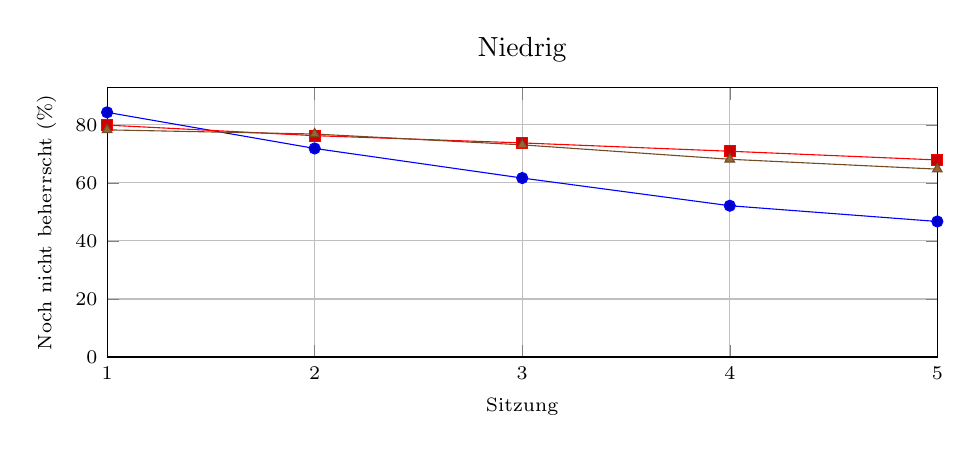
\begin{tikzpicture}
\begin{axis}[width=\linewidth,height=5cm,title={Niedrig},xlabel={Sitzung},ylabel={Noch nicht beherrscht (\%)},xmin=1,xmax=5,xtick={1,...,5},ymin=0,grid=major,tick label style={font=\scriptsize},label style={font=\scriptsize}]
\addplot+[mark=*] coordinates {(1,84.29999999999993) (2,71.86666666666667) (3,61.66666666666668) (4,52.13333333333333) (5,46.69999999999999)};
\addplot+[mark=square*] coordinates {(1,79.89999999999998) (2,76.26666666666664) (3,73.76666666666667) (4,70.89999999999999) (5,67.90000000000002)};
\addplot+[mark=triangle*] coordinates {(1,78.26666666666661) (2,76.83333333333331) (3,73.1) (4,68.13333333333337) (5,64.73333333333336)};
\end{axis}
\end{tikzpicture}
\end{minipage}\hfill
\begin{minipage}{0.48\textwidth}\centering
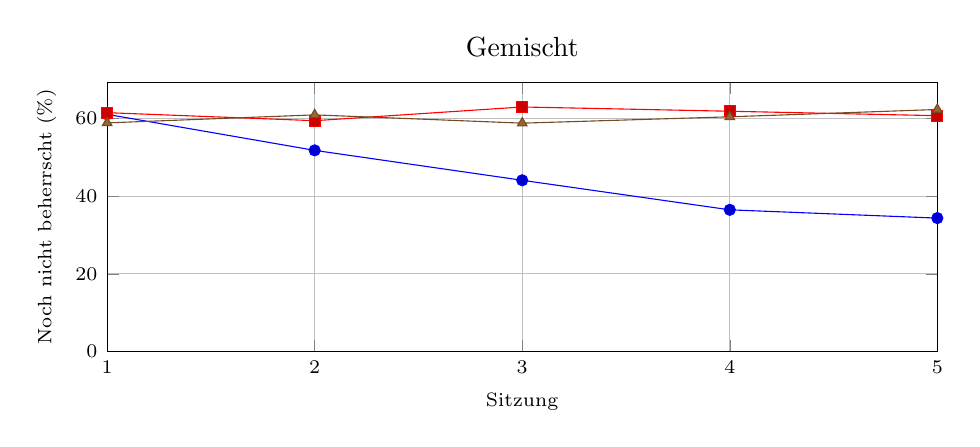
\begin{tikzpicture}
\begin{axis}[width=\linewidth,height=5cm,title={Gemischt},xlabel={Sitzung},ylabel={Noch nicht beherrscht (\%)},xmin=1,xmax=5,xtick={1,...,5},ymin=0,grid=major,tick label style={font=\scriptsize},label style={font=\scriptsize}]
\addplot+[mark=*] coordinates {(1,61.066666666666706) (2,51.800000000000004) (3,44.09999999999999) (4,36.49999999999999) (5,34.366666666666674)};
\addplot+[mark=square*] coordinates {(1,61.5) (2,59.43333333333336) (3,62.96666666666668) (4,61.86666666666669) (5,60.72194188619973)};
\addplot+[mark=triangle*] coordinates {(1,58.86666666666668) (2,60.93333333333334) (3,58.80000000000003) (4,60.43333333333335) (5,62.317266922094504)};
\end{axis}
\end{tikzpicture}
\end{minipage}\par\medskip
\begin{minipage}{0.48\textwidth}\centering
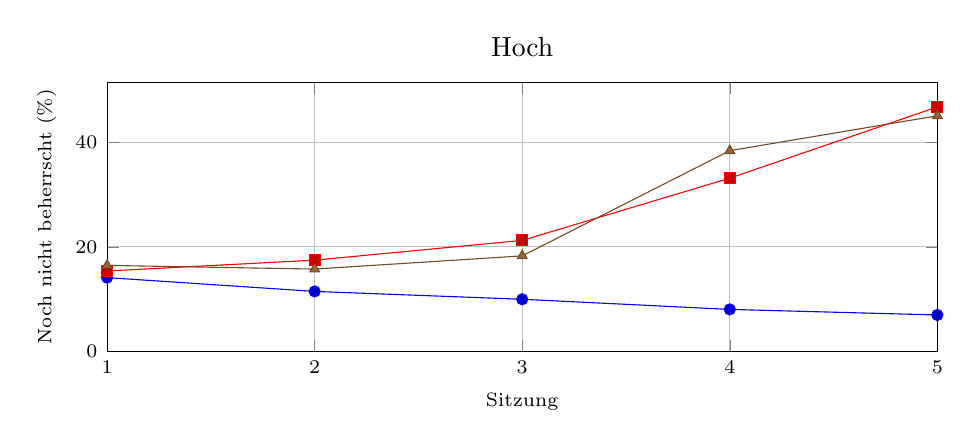
\begin{tikzpicture}
\begin{axis}[width=\linewidth,height=5cm,title={Hoch},xlabel={Sitzung},ylabel={Noch nicht beherrscht (\%)},xmin=1,xmax=5,xtick={1,...,5},ymin=0,grid=major,tick label style={font=\scriptsize},label style={font=\scriptsize}]
\addplot+[mark=*] coordinates {(1,14.133333333333315) (2,11.49999999999999) (3,9.999999999999995) (4,8.066666666666663) (5,6.9999999999999964)};
\addplot+[mark=square*] coordinates {(1,15.399999999999986) (2,17.466666666666654) (3,21.23563218390805) (4,33.11497488073324) (5,46.70843776106933)};
\addplot+[mark=triangle*] coordinates {(1,16.466666666666644) (2,15.766666666666648) (3,18.283678160919525) (4,38.36218458692412) (5,45.028583137135776)};
\end{axis}
\end{tikzpicture}
\end{minipage}\hfill
\begin{minipage}{0.48\textwidth}\centering
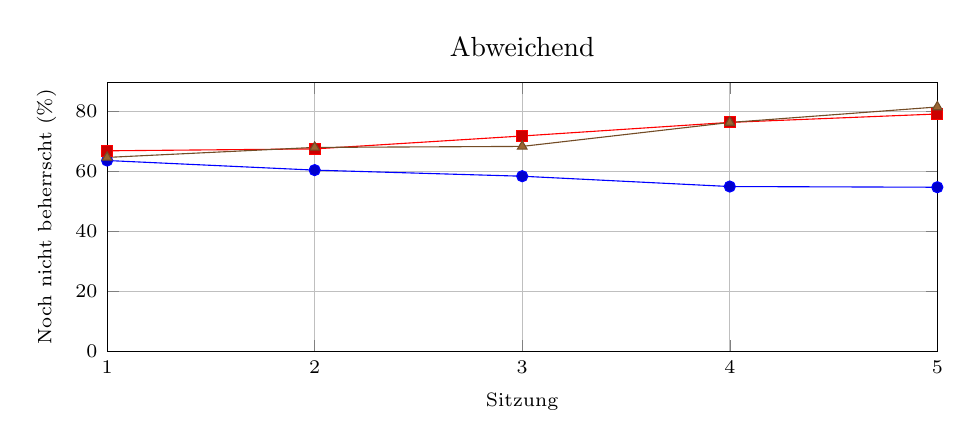
\begin{tikzpicture}
\begin{axis}[width=\linewidth,height=5cm,title={Abweichend},xlabel={Sitzung},ylabel={Noch nicht beherrscht (\%)},xmin=1,xmax=5,xtick={1,...,5},ymin=0,grid=major,tick label style={font=\scriptsize},label style={font=\scriptsize}]
\addplot+[mark=*] coordinates {(1,63.666666666666686) (2,60.46666666666668) (3,58.43333333333334) (4,55.00000000000003) (5,54.76666666666667)};
\addplot+[mark=square*] coordinates {(1,66.89999999999998) (2,67.53333333333333) (3,71.83333333333337) (4,76.36666666666667) (5,79.16666666666664)};
\addplot+[mark=triangle*] coordinates {(1,64.70000000000002) (2,68.03333333333335) (3,68.36666666666666) (4,76.3333333333333) (5,81.5025641025641)};
\end{axis}
\end{tikzpicture}
\end{minipage}\par\medskip
\par\smallskip\footnotesize Blau/Kreise: Zufall; Rot/Quadrate: Bewertungen und Lernstand; Braun/Dreiecke: Informationsgewinn.}
\newcommand{\EvaluationCoveragePlot}{%
\begin{minipage}{0.48\textwidth}\centering
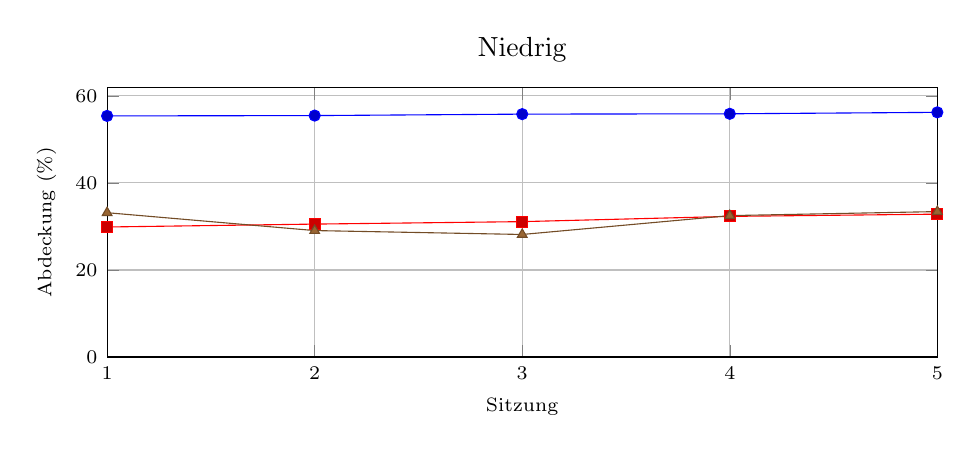
\begin{tikzpicture}
\begin{axis}[width=\linewidth,height=5cm,title={Niedrig},xlabel={Sitzung},ylabel={Abdeckung (\%)},xmin=1,xmax=5,xtick={1,...,5},ymin=0,grid=major,tick label style={font=\scriptsize},label style={font=\scriptsize}]
\addplot+[mark=*] coordinates {(1,55.38461538461538) (2,55.46153846153848) (3,55.794871794871824) (4,55.87179487179487) (5,56.20512820512822)};
\addplot+[mark=square*] coordinates {(1,29.871794871794837) (2,30.538461538461505) (3,31.102564102564063) (4,32.30769230769227) (5,32.82051282051278)};
\addplot+[mark=triangle*] coordinates {(1,33.15384615384611) (2,29.051282051282023) (3,28.153846153846118) (4,32.48717948717944) (5,33.41025641025637)};
\end{axis}
\end{tikzpicture}
\end{minipage}\hfill
\begin{minipage}{0.48\textwidth}\centering
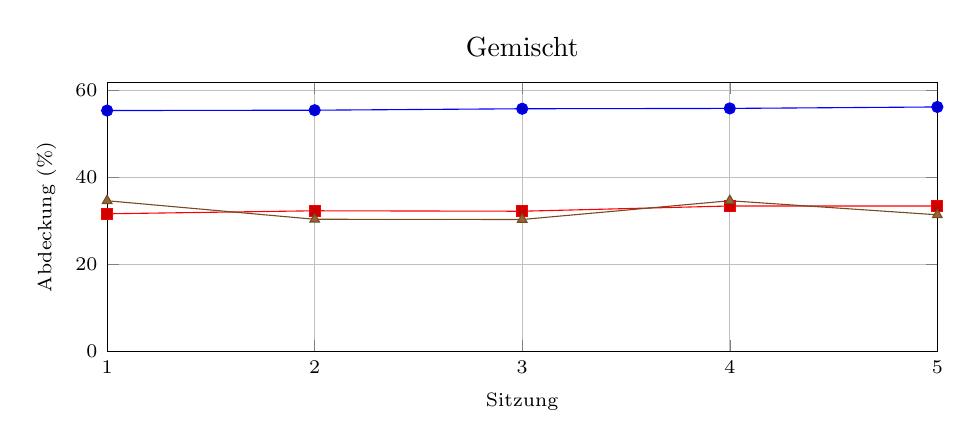
\begin{tikzpicture}
\begin{axis}[width=\linewidth,height=5cm,title={Gemischt},xlabel={Sitzung},ylabel={Abdeckung (\%)},xmin=1,xmax=5,xtick={1,...,5},ymin=0,grid=major,tick label style={font=\scriptsize},label style={font=\scriptsize}]
\addplot+[mark=*] coordinates {(1,55.38461538461538) (2,55.46153846153848) (3,55.794871794871824) (4,55.87179487179487) (5,56.20512820512822)};
\addplot+[mark=square*] coordinates {(1,31.666666666666625) (2,32.35897435897432) (3,32.25641025641021) (4,33.46153846153842) (5,33.461538461538424)};
\addplot+[mark=triangle*] coordinates {(1,34.66666666666662) (2,30.410256410256377) (3,30.358974358974322) (4,34.666666666666615) (5,31.43589743589739)};
\end{axis}
\end{tikzpicture}
\end{minipage}\par\medskip
\begin{minipage}{0.48\textwidth}\centering
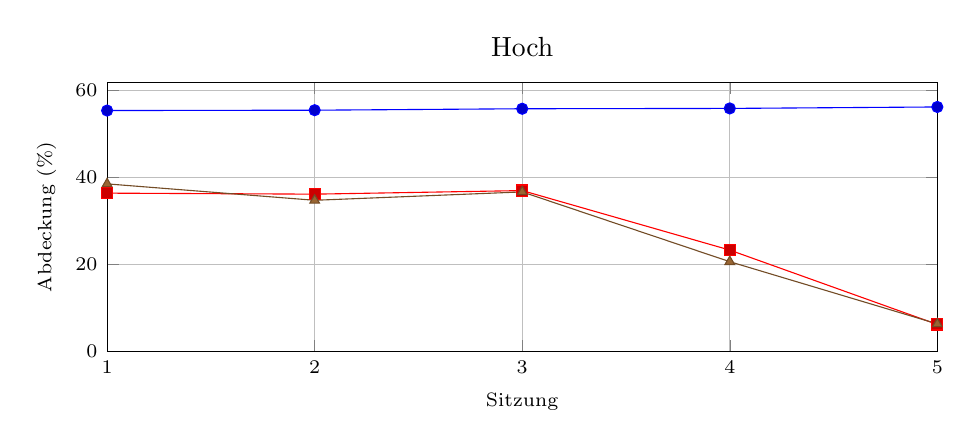
\begin{tikzpicture}
\begin{axis}[width=\linewidth,height=5cm,title={Hoch},xlabel={Sitzung},ylabel={Abdeckung (\%)},xmin=1,xmax=5,xtick={1,...,5},ymin=0,grid=major,tick label style={font=\scriptsize},label style={font=\scriptsize}]
\addplot+[mark=*] coordinates {(1,55.38461538461538) (2,55.46153846153848) (3,55.794871794871824) (4,55.87179487179487) (5,56.20512820512822)};
\addplot+[mark=square*] coordinates {(1,36.41025641025637) (2,36.17948717948713) (3,36.99999999999997) (4,23.333333333333304) (5,6.251800633823098)};
\addplot+[mark=triangle*] coordinates {(1,38.53846153846151) (2,34.76923076923073) (3,36.69230769230766) (4,20.66666666666664) (5,6.383547008547001)};
\end{axis}
\end{tikzpicture}
\end{minipage}\hfill
\begin{minipage}{0.48\textwidth}\centering
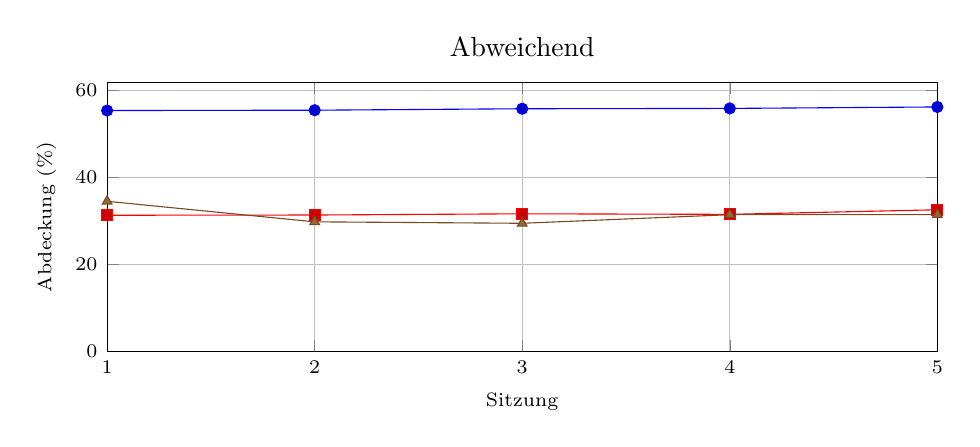
\begin{tikzpicture}
\begin{axis}[width=\linewidth,height=5cm,title={Abweichend},xlabel={Sitzung},ylabel={Abdeckung (\%)},xmin=1,xmax=5,xtick={1,...,5},ymin=0,grid=major,tick label style={font=\scriptsize},label style={font=\scriptsize}]
\addplot+[mark=*] coordinates {(1,55.38461538461538) (2,55.46153846153848) (3,55.794871794871824) (4,55.87179487179487) (5,56.20512820512822)};
\addplot+[mark=square*] coordinates {(1,31.33333333333329) (2,31.384615384615344) (3,31.666666666666625) (4,31.538461538461494) (5,32.58974358974355)};
\addplot+[mark=triangle*] coordinates {(1,34.5384615384615) (2,29.82051282051279) (3,29.48717948717945) (4,31.461538461538417) (5,31.487179487179446)};
\end{axis}
\end{tikzpicture}
\end{minipage}\par\medskip
\par\smallskip\footnotesize Blau/Kreise: Zufall; Rot/Quadrate: Bewertungen und Lernstand; Braun/Dreiecke: Informationsgewinn.}
\newcommand{\EvaluationEndpointTable}{%
\begin{tabular}{lrrrrrrrrr}
\hline
& \multicolumn{3}{c}{Zufall} & \multicolumn{3}{c}{Bewertungen + Lernstand} & \multicolumn{3}{c}{Informationsgewinn} \\
Situation & Aufgaben & Abdeckung & Brier & Aufgaben & Abdeckung & Brier & Aufgaben & Abdeckung & Brier \\
\hline
Niedrig & $150{,}0$ & $95{,}7$ & $0{,}1461$ & $150{,}0$ & $91{,}5$ & $0{,}1566$ & $150{,}0$ & $89{,}7$ & $0{,}1364$ \\
Gemischt & $150{,}0$ & $95{,}7$ & $0{,}1189$ & $149{,}8$ & $96{,}4$ & $0{,}1124$ & $149{,}8$ & $95{,}8$ & $0{,}1039$ \\
Hoch & $150{,}0$ & $95{,}7$ & $0{,}0615$ & $110{,}8$ & $100{,}0$ & $0{,}0216$ & $110{,}5$ & $100{,}0$ & $0{,}0216$ \\
Abweichend & $150{,}0$ & $95{,}7$ & $0{,}1756$ & $150{,}0$ & $93{,}0$ & $0{,}2387$ & $150{,}0$ & $90{,}8$ & $0{,}2215$ \\
\hline
\end{tabular}}
